%----------------------------------------------------------------------------------------
%	HOMEWORK ASSIGNMENT CSCI 5521
%----------------------------------------------------------------------------------------

%----------------------------------------------------------------------------------------
%	PROLOUGE 
%----------------------------------------------------------------------------------------
\documentclass[a4paper, 11pt]{article}
\usepackage[scale=0.85]{geometry} 		% Reduce document margins
\usepackage{hyperref} 					% Required for hyperlinks i.e. e-mail %
\usepackage{titlesec} 					% Used to customize the \section command
\usepackage[T1]{fontenc}				% Used to have both Bold and Small caps in heading
\usepackage{amsmath}					% Used to write equations
\usepackage{amssymb}					% Used to write math symbols e.g. R = real number set
\usepackage{autobreak}
\usepackage{graphicx}					% Used to include images
\usepackage{tabularx} 					% For custom table %

%----------------------------------------------------------------------------------------
%	CUSTOM MACRO DEFINITION AND ENVIRONMENT MODIFICATION
%----------------------------------------------------------------------------------------
\titleformat{\section}{\bfseries\Large\scshape\filcenter}{}{0em}{}[{\titlerule[1pt]}] % Text formatting of sections
\titlespacing{\section}{0pt}{3pt}{3pt} % Spacing around sections
\pagestyle{empty} % Removes page numbering
\newcommand{\xVec}{\ensuremath{\boldsymbol{x}}}
\newcommand{\muVec}{\ensuremath{\boldsymbol{\mu}}}
\newcommand{\mVec}{\ensuremath{\boldsymbol{m}}}
\newcommand{\sVec}{\ensuremath{\boldsymbol{S}}}
\newcommand{\SigmaVec}{\ensuremath{\boldsymbol{\Sigma}}}
%----------------------------------------------------------------------------------------
%	MAIN BODY
%----------------------------------------------------------------------------------------
\begin{document}
	%----------------------------------------------------------------------------------------
%	HEADER
%----------------------------------------------------------------------------------------
\section{HW 4}
\begin{tabularx}{\textwidth}{l}
	\hspace*{-0.8cm}\large\textsc{Arnab Dey}\\
	\hspace*{-0.8cm}Student ID: 5563169\\
	\hspace*{-0.8cm}Email: dey00011@umn.edu\\
\end{tabularx}
\bigskip
\par
    %----------------------------------------------------------------------------------------
%	SOLUTION 1.a
%----------------------------------------------------------------------------------------
\subsection*{Solution 1.a}
Fig.~\ref{fig:q1_a} shows the decision boundary for the dummy data created in Q1.a. The error rate on this dataset is $0\%$.
\begin{figure}[h!]
	\centering
	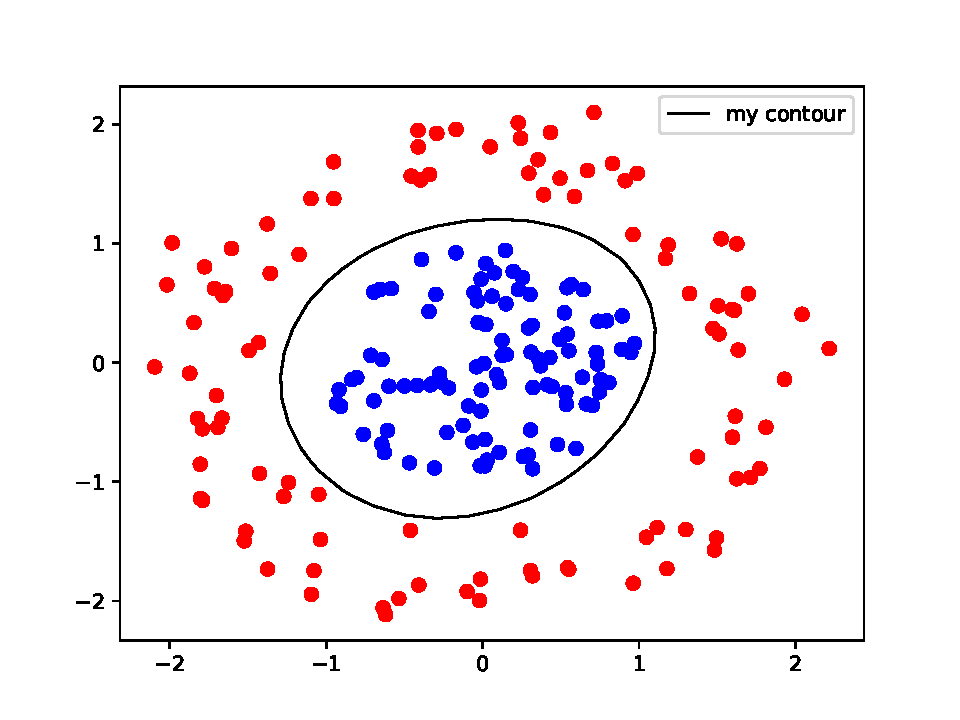
\includegraphics[scale=0.5]{q1_a_my_contour.pdf}
	\caption{Classification with polynomial kernel of degree $3$}
	\label{fig:q1_a}
\end{figure}
%----------------------------------------------------------------------------------------
%	SOLUTION 1.b
%----------------------------------------------------------------------------------------
\subsection*{Solution 1.b}
Fig.~\ref{fig:q1_b} shows the decision boundary returned by 'svc' function of 'SVM' module of 'sklearn' package with the same kernel as previous one.
\begin{figure}[h!]
	\centering
	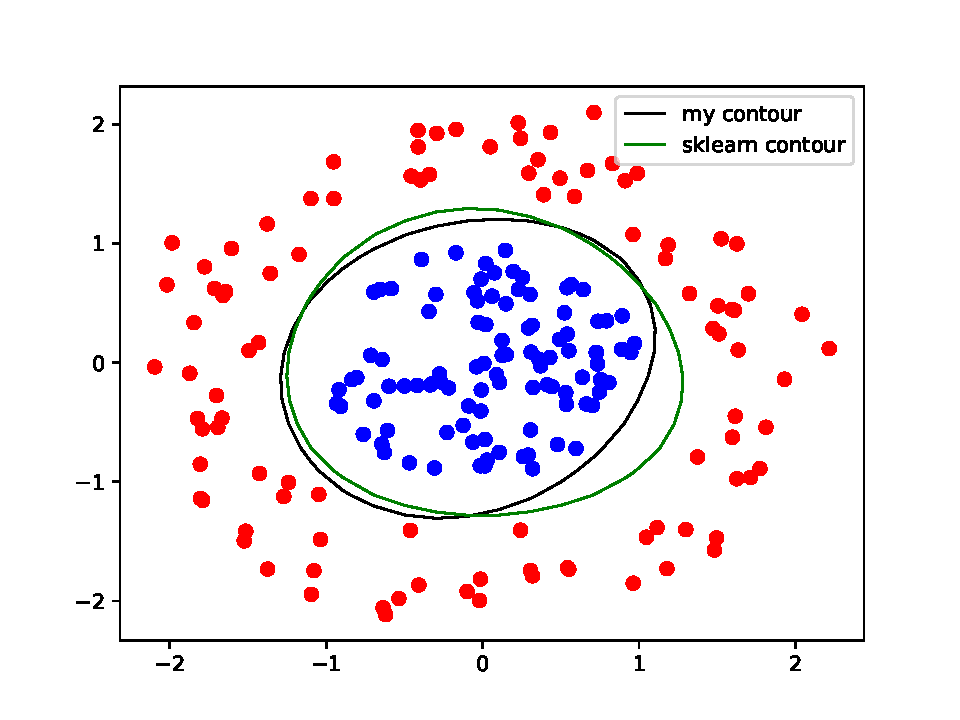
\includegraphics[scale=0.5]{q1_a_svc_contour.pdf}
	\caption{Classification with polynomial kernel of degree $3$ with scikit-learn module}
	\label{fig:q1_b}
\end{figure}
Fig.~\ref{fig:q1_b} shows that the decision boundary returned by 'sklearn' is better because of the additional regularization parameter used by 'sklearn' package. Fig.~\ref{fig:q1_b} shows the decision boundary for regularization parameter $C = 0.05$.
\begin{figure}[h!]
	\centering
	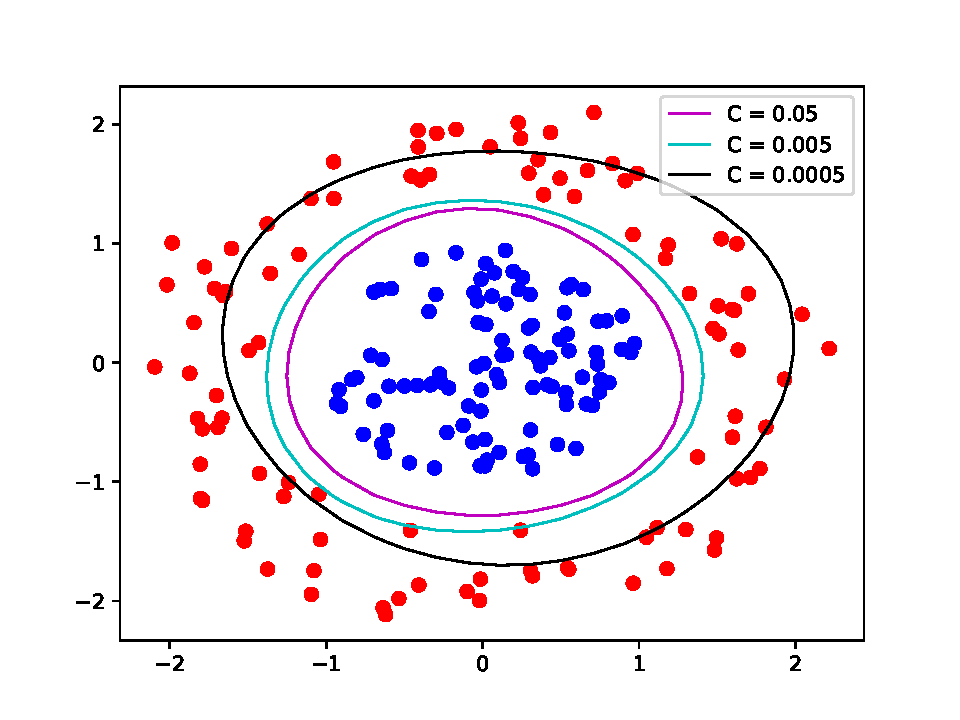
\includegraphics[scale=0.5]{q1_a_svc_c_effect.pdf}
	\caption{Classification with polynomial kernel of degree $3$ with different regularization parameter $C$ of scikit-learn module}
	\label{fig:q1_b1}
\end{figure}
Fig.~\ref{fig:q1_b1} shows that decreasing the regularization parameter makes the decision boundary wider thus causing more error on training set. On the other hand, increasing the regularization parameter shrinks the decision boundary and too much increment will also cause larger training error.
%----------------------------------------------------------------------------------------
%	SOLUTION 1.c
%----------------------------------------------------------------------------------------
\subsection*{Solution 1.c}
The following table shows the training and test error rates on both 'optdigits49' and 'optdigits79' dataset.
\begin{table}[h!]
	\begin{center}
		\begin{tabular}{||c | c | c ||} 
			\hline
			Dataset & Training error (\%) & Test error (\%)\\ [0.5ex] 
			\hline\hline
			optdigits49 & 0.473 & 3.169\\ [0.5ex]
			\hline
			optdigits79 & 0.355 & 0.709\\ [1ex]
			\hline
		\end{tabular}
	\end{center}
	\caption{Q1.c: Error-rate on subset of optdigit dataset}
\end{table}
    %----------------------------------------------------------------------------------------
%	SOLUTION 2.a
%----------------------------------------------------------------------------------------
\subsection*{Solution 2.a}
Error rate on training and validation dataset for different hidden units are shown in the following table:
\begin{table}[h!]
	\begin{center}
		\begin{tabular}{||c | c | c | c | c | c | c ||} 
			\hline
			Hidden units & 3 & 6 & 9 & 12 & 15 & 18 \\ [0.5ex] 
			\hline\hline
			Training error(\%) & 15.91 & 1.38 & 0.21 & 0.05 & 0.05 & 0.05 \\ [0.5ex]
			\hline \hline
			Validation error(\%) & 19.27 & 7.21 & 3.58 & 3.26 & 3.15 & 3.58 \\ [1ex]
			\hline
		\end{tabular}
	\end{center}
	\caption{Q2.a: Error-rate Vs. hidden units table}
\end{table}
The plot is shown Fig.~\ref{fig:tv_error_2a}
\begin{figure}[h!]
	\centering
	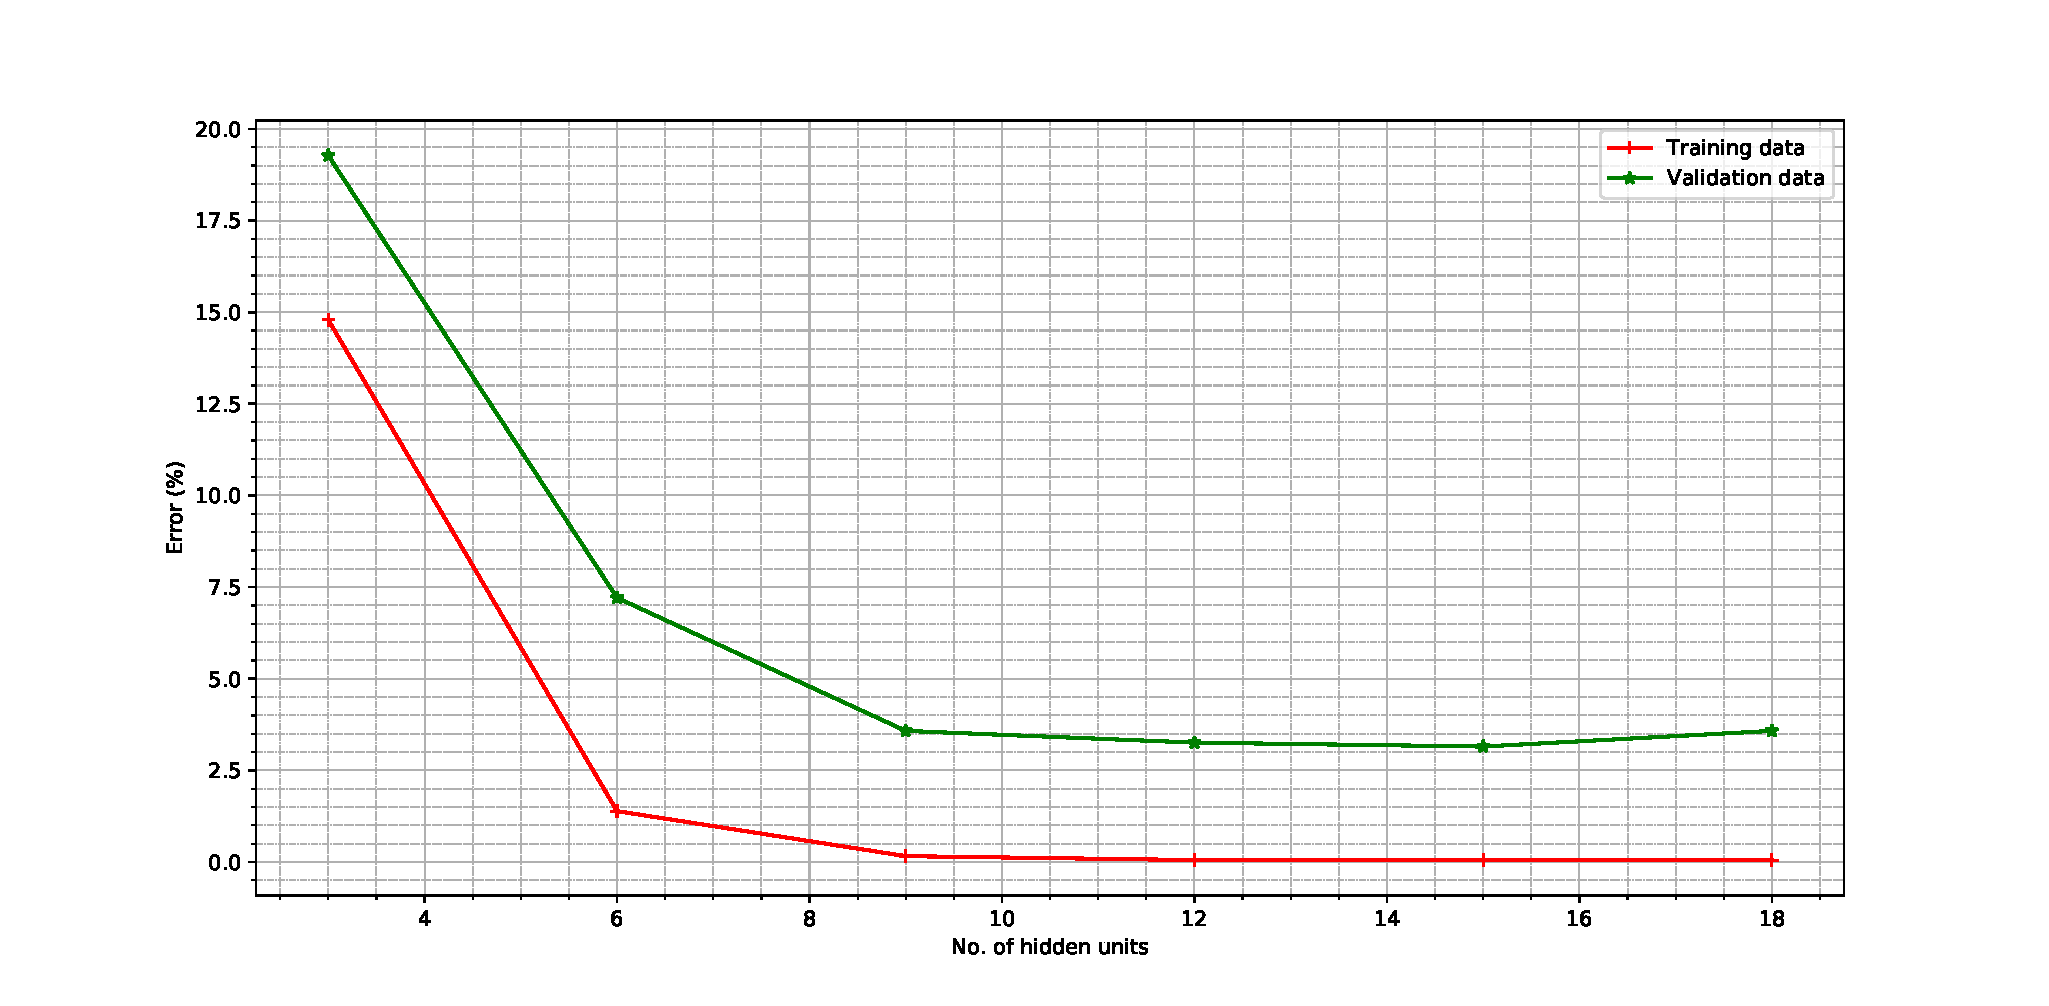
\includegraphics[scale=0.5]{2a_tv_error.pdf}
	\caption{Error Vs. hidden units plot for Optdigits training and validation data}
	\label{fig:tv_error_2a}
\end{figure}
\newline
As we can see from Fig.~\ref{fig:tv_error_2a}, both training and validation error decreases with increase in number of hidden units. But error on validation data with 18 hidden units gets slightly higher compared to 15 hidden units. This implies over-trained MLP. Therefore, for best results, we should choose 15 hidden units.

Error rate on test data with 15 hidden units is shown in the following table:
\begin{table}[h!]
	\begin{center}
		\begin{tabular}{||c | c ||} 
			\hline
			Hidden units & 15 \\ [0.5ex] 
			\hline\hline
			Test error(\%) & 4.1\\ [1ex]
			\hline
		\end{tabular}
	\end{center}
	\caption{Q2.a: Error-rate on test data}
\end{table}
%----------------------------------------------------------------------------------------
%	SOLUTION 2.b
%----------------------------------------------------------------------------------------
\subsection*{Solution 2.b}
Hidden units used = 15. Hidden representation with 2 principal components is shown in Fig.~\ref{fig:pca2_2b}, and with 3 principal components is shown in Fig.~\ref{fig:pca3_2b}.
\begin{figure}[h!]
	\centering
	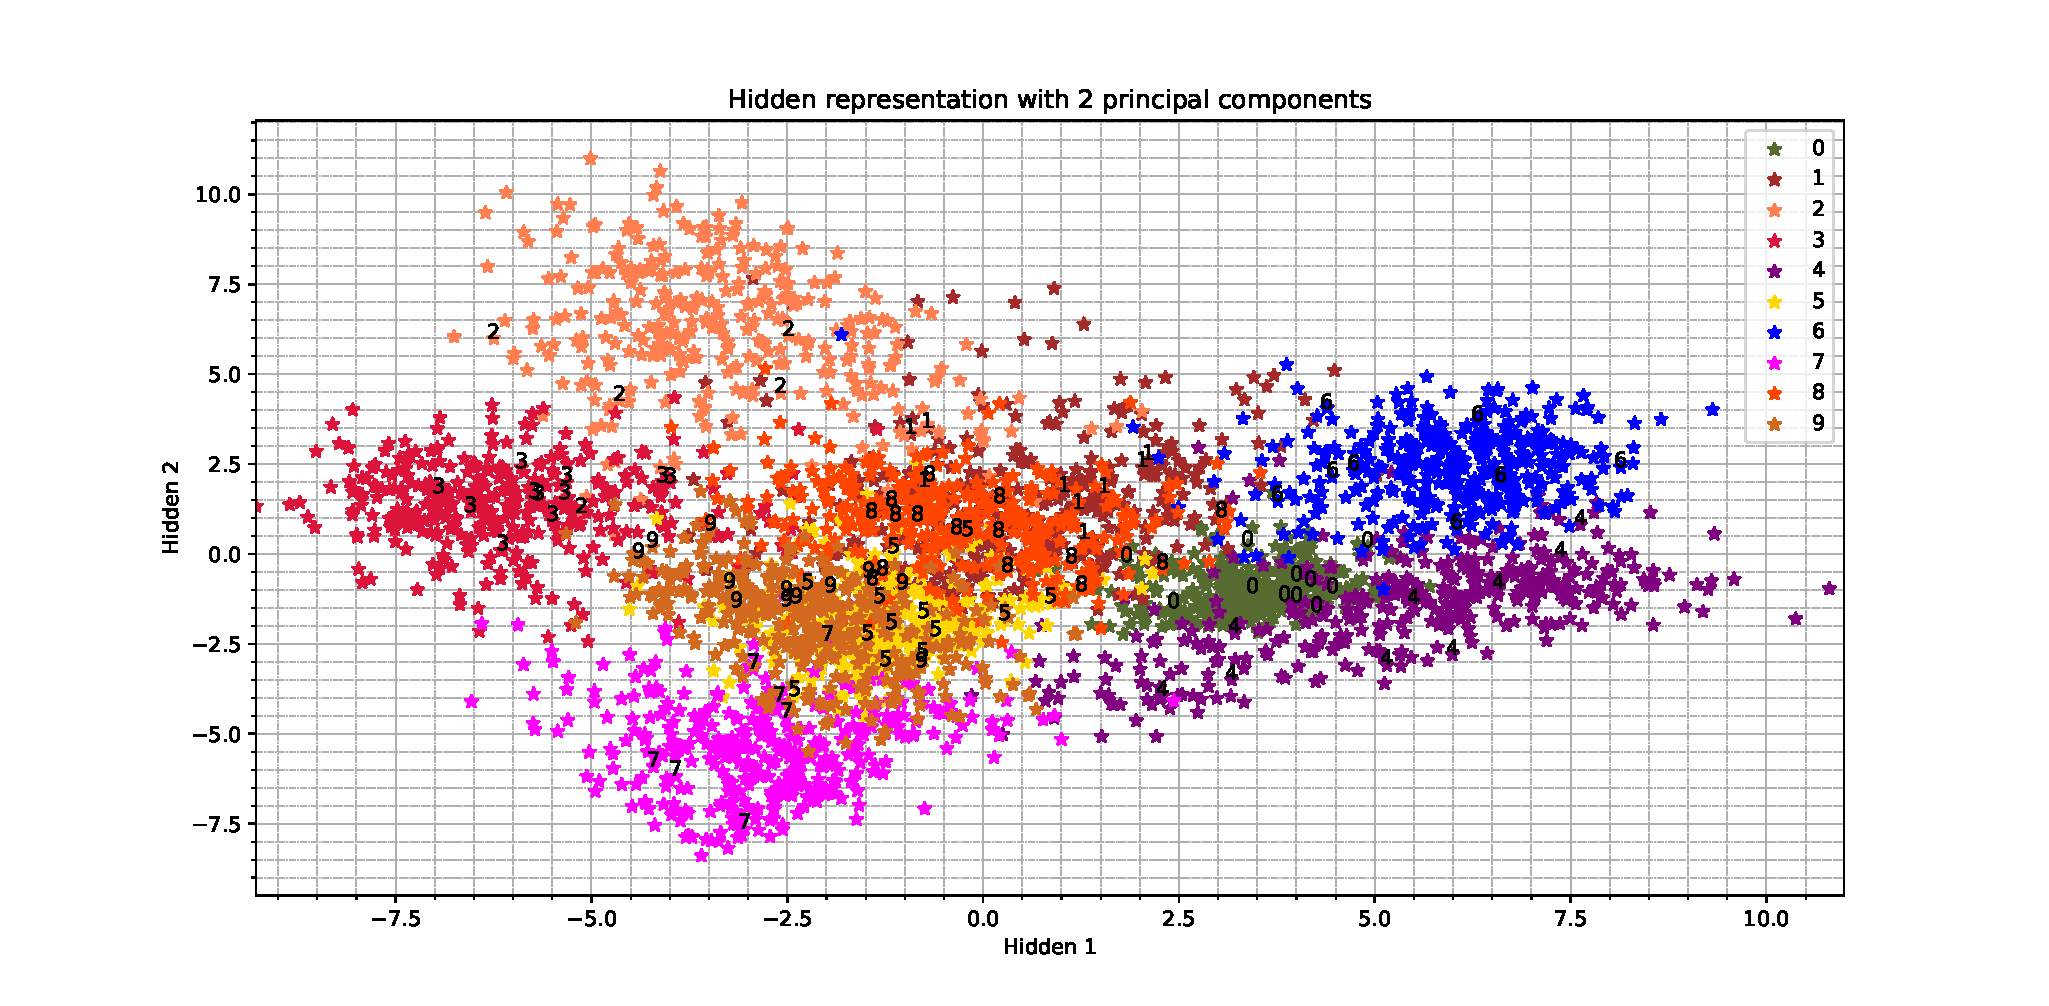
\includegraphics[scale=0.5]{2b_pca2.pdf}
	\caption{Hidden representation with 2 principal components on training and validation data}
	\label{fig:pca2_2b}
\end{figure}
\begin{figure}[h!]
	\centering
	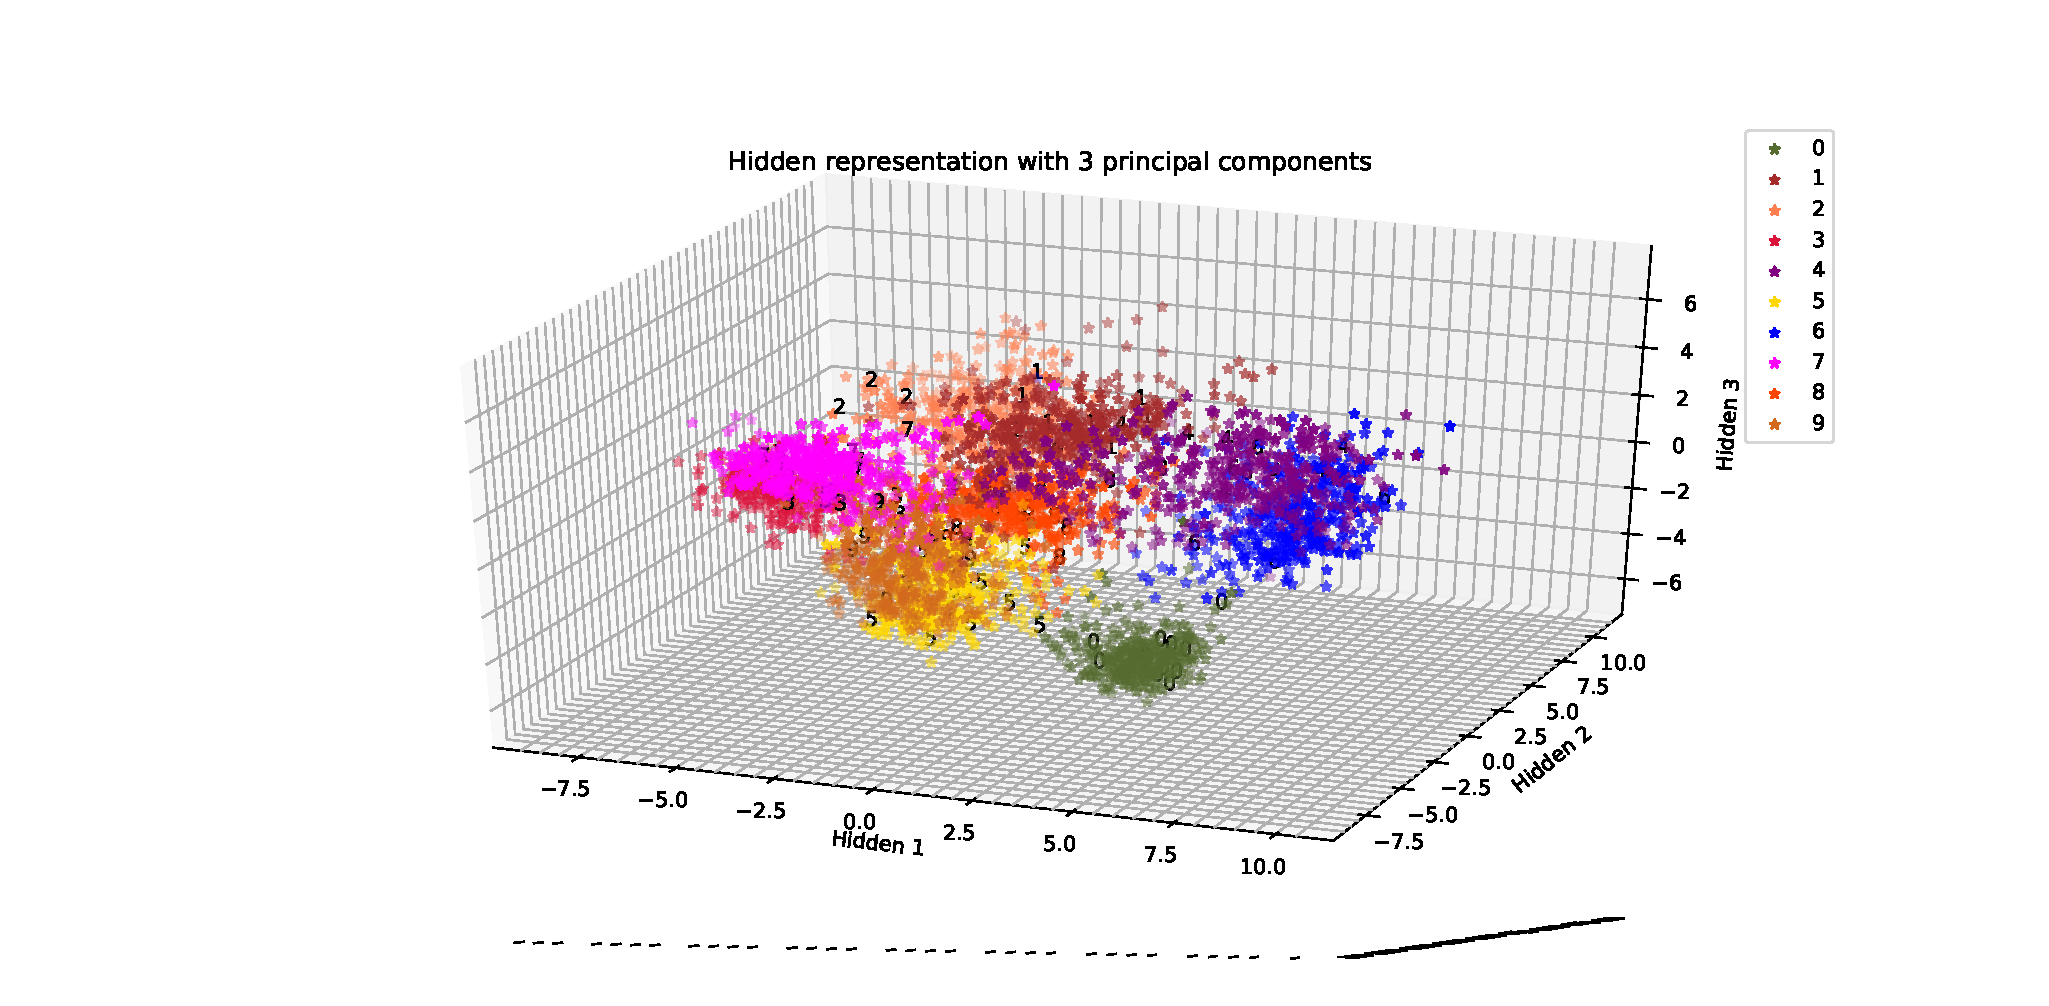
\includegraphics[scale=0.5]{2b_pca3.pdf}
	\caption{Hidden representation with 3 principal components on training and validation data}
	\label{fig:pca3_2b}
\end{figure}
Thus from Fig.~\ref{fig:pca2_2b} and Fig.~\ref{fig:pca3_2b}, we can see that PCA with 3 principal components provide better separation than with 2 principal components. This happens as number of PCA components behaves as a representation of number of units in the hidden layer.
    %----------------------------------------------------------------------------------------
%	SOLUTION 3
%----------------------------------------------------------------------------------------
\subsection*{Solution 3.a}
The mean face is shown in Fig.\ref{fig:mean_face}
\begin{figure}[h!]
	\centering
	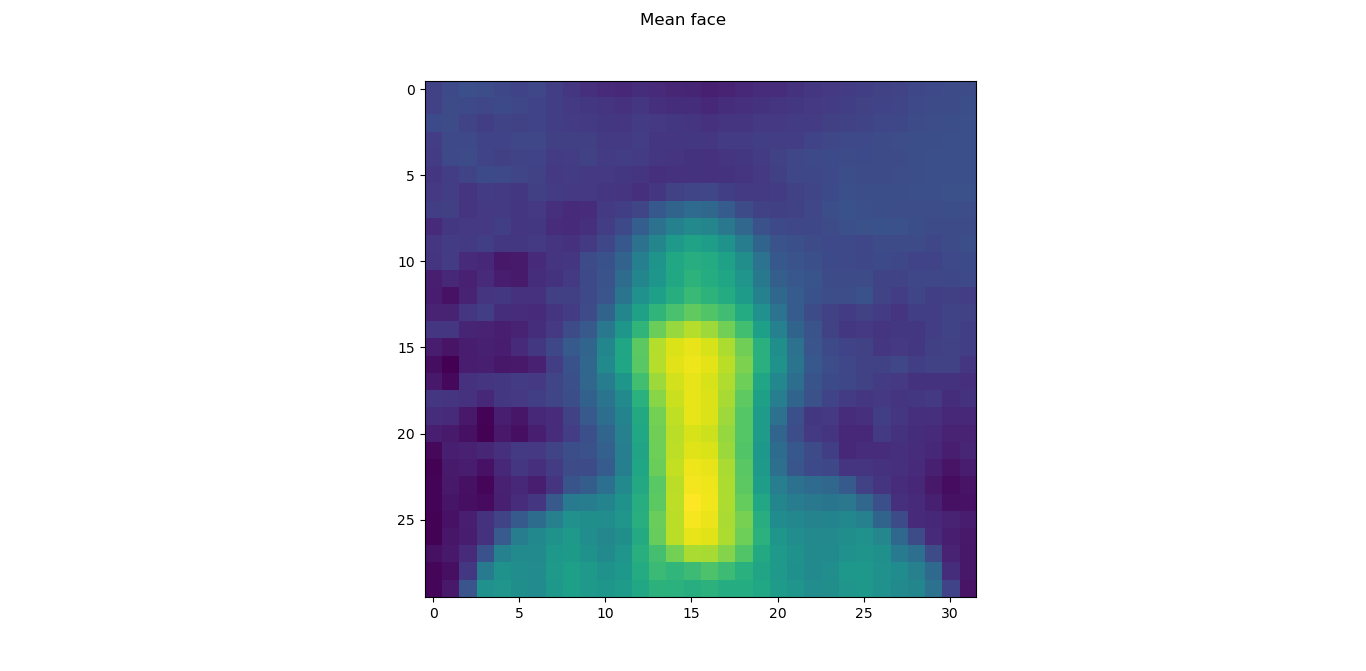
\includegraphics[scale=0.5]{mean_face}
	\caption{Mean face}
	\label{fig:mean_face}
\end{figure}
The first 5 eigen-faces are shown in Fig.\ref{fig:eig_faces}
\newpage
\begin{figure}[h!]
	\centering
	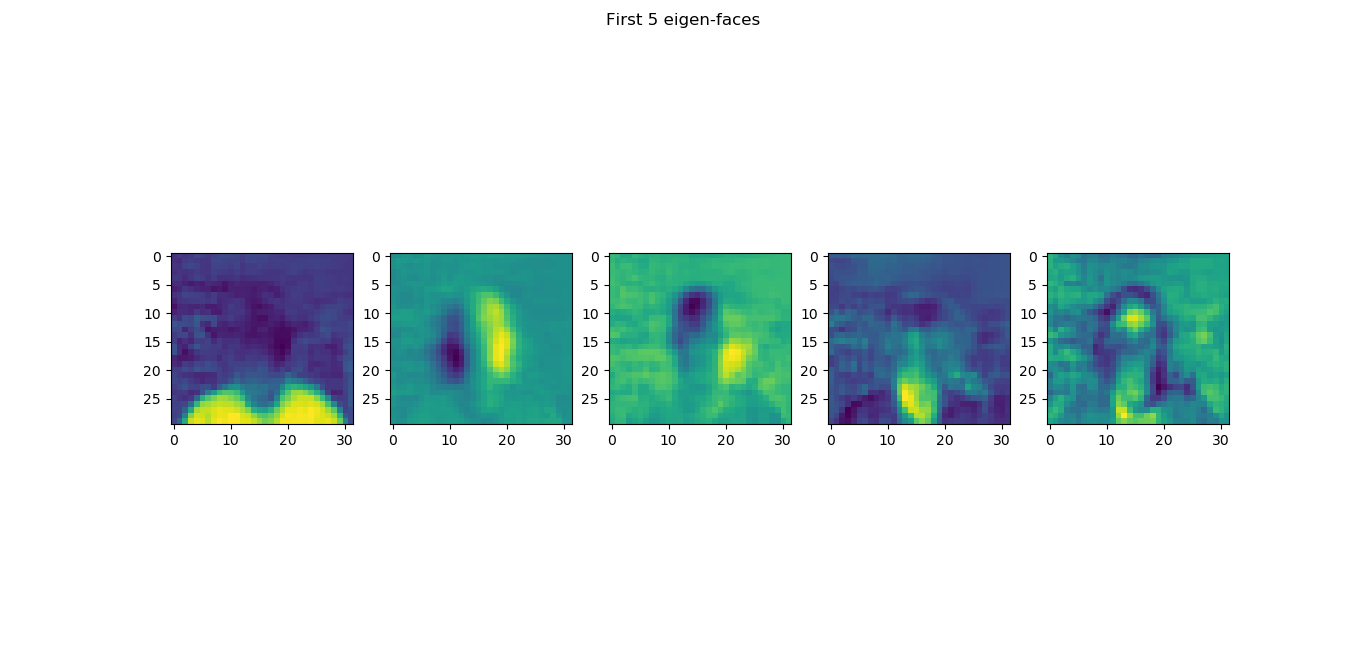
\includegraphics[scale=0.5]{eig_faces}
	\caption{First 5 eigen-faces}
	\label{fig:eig_faces}
\end{figure}
\subsection*{Solution 3.b}
We performed PCA on face training data and found the following proportion of variance plot:
\begin{figure}[h!]
	\centering
	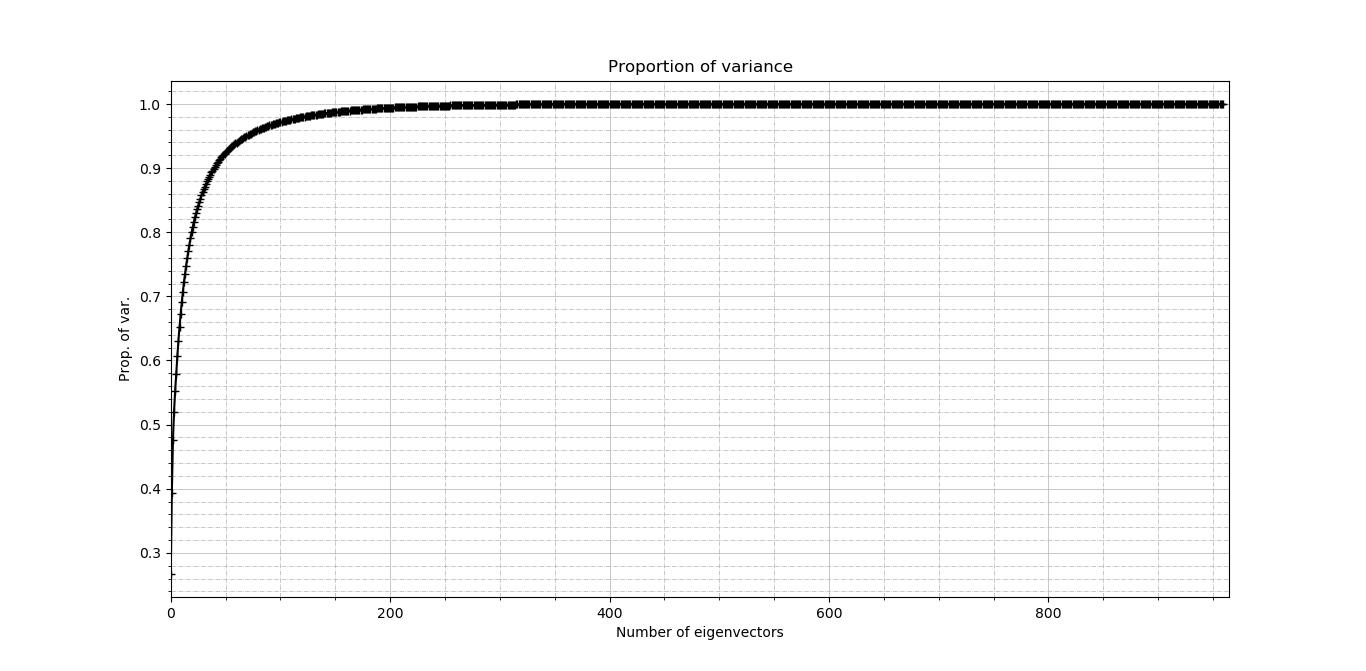
\includegraphics[scale=0.5]{pov_3b}
	\caption{Proportion of variance plot for face training data}
	\label{fig:pov_3b}
\end{figure}
\newline
We can see from Fig.\ref{fig:pov_3b} that the minimum number of eigenvectors that explain at least 90\% of the variance is 40.
\newline
Therefore, we used 40 principal components for PCA and reduced the dimension of the original face data to 40. Then, we used KNN on this reduced dimension face test data. The following table shows the error rates for different k in k-nearest neighbor algorithm on reduced face test data.
\begin{table}[h!]
	\begin{center}
		\begin{tabular}{||c | c | c | c | c ||} 
			\hline
			k & 1 & 3 & 5 & 7 \\ [0.5ex] 
			\hline\hline
			Error rate(\%) & 10.483 & 24.193 & 39.516 & 39.516 \\ [1ex]
			\hline
		\end{tabular}
	\end{center}
	\caption{Q3.b: Error-rate Vs. k table}
\end{table}
\subsection*{Solution 3.c}
\begin{figure}[h!]
	\centering
	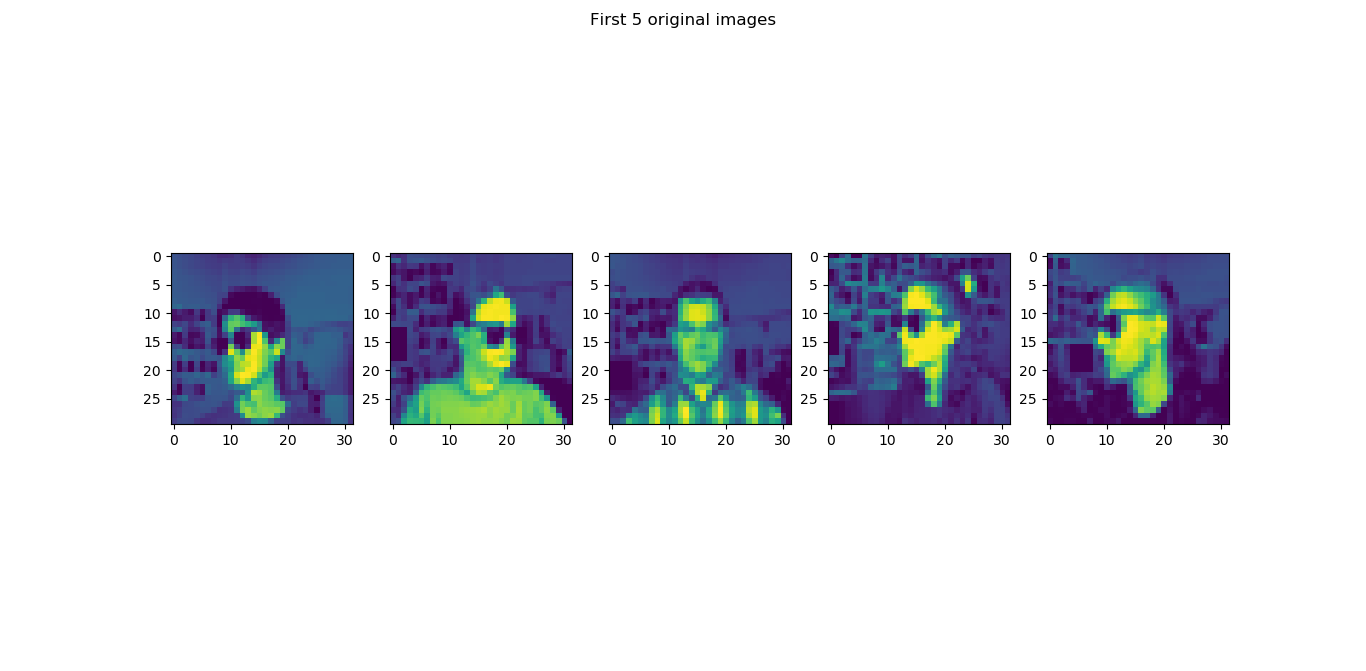
\includegraphics[scale=0.5]{face_orig}
	\caption{Original first 5 faces from training data}
	\label{fig:face_orig}
\end{figure}
\begin{figure}[h!]
	\centering
	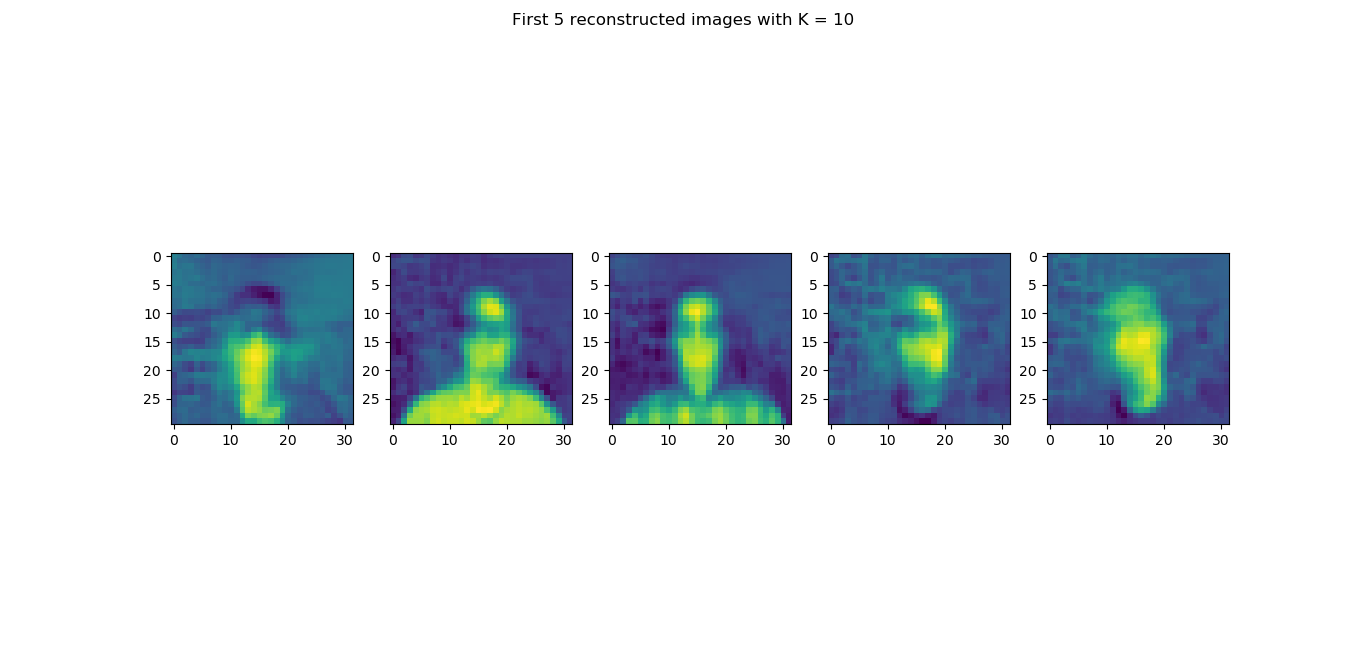
\includegraphics[scale=0.5]{face_pca_10}
	\caption{First 5 reconstructed faces using 10 principal components}
	\label{fig:face_pca_10}
\end{figure}
\begin{figure}[h!]
	\centering
	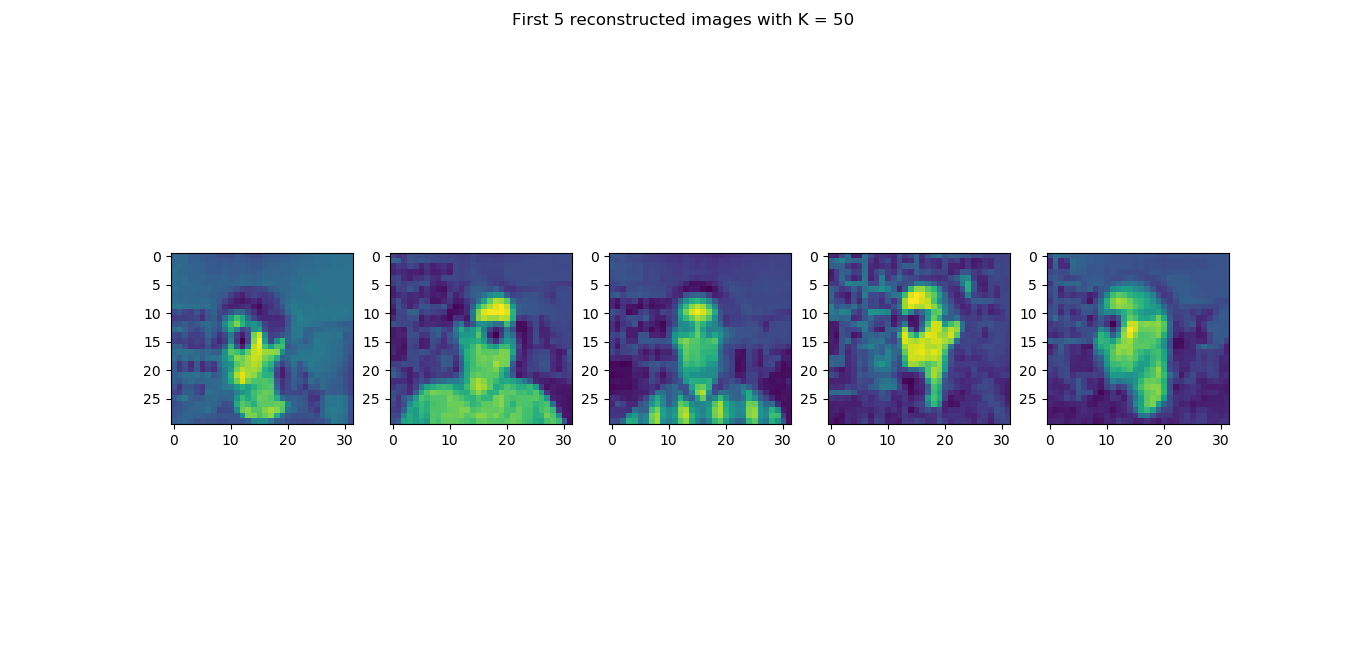
\includegraphics[scale=0.5]{face_pca_50}
	\caption{First 5 reconstructed faces using 50 principal components}
	\label{fig:face_pca_50}
\end{figure}
\begin{figure}[h!]
	\centering
	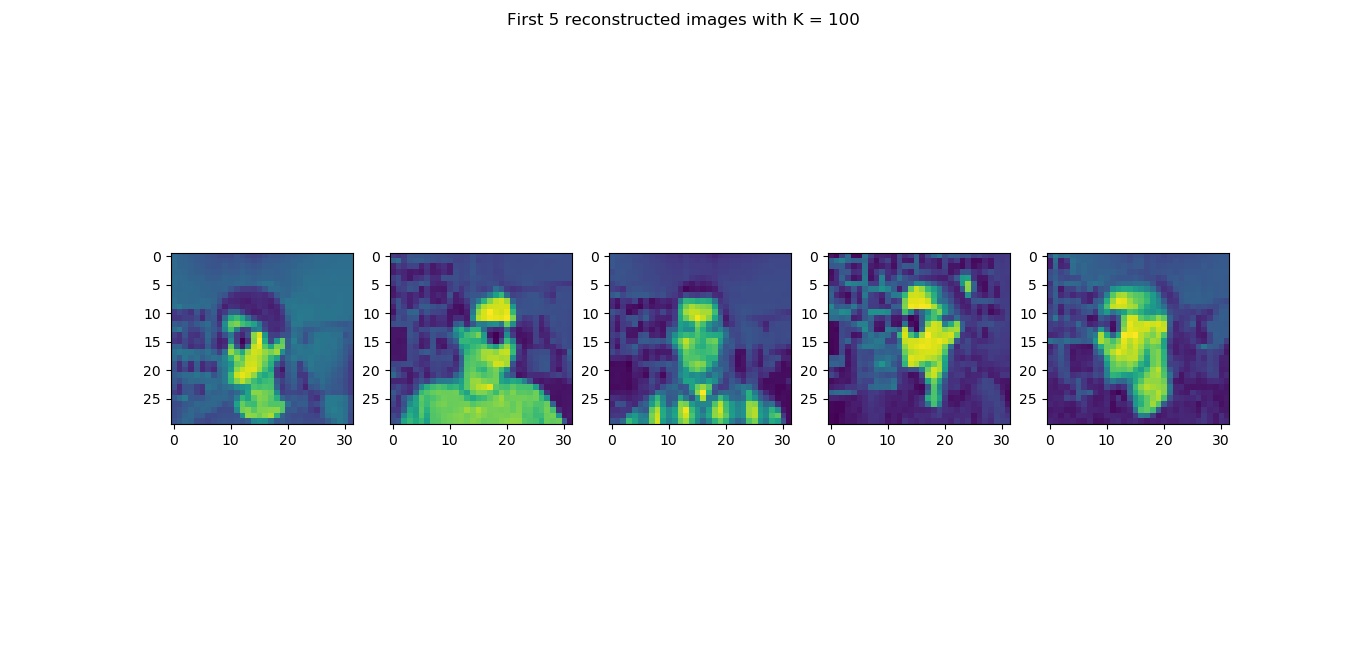
\includegraphics[scale=0.5]{face_pca_100}
	\caption{First 5 reconstructed faces using 100 principal components}
	\label{fig:face_pca_100}
\end{figure}
\newpage
Thus we can see that as we increase the number of principal components, reconstructed images become closer to the original images but at a cost of increased complexity and processing time.
    %%----------------------------------------------------------------------------------------
%	SOLUTION 3
%----------------------------------------------------------------------------------------
\subsection*{Solution 3.a}
The mean face is shown in Fig.\ref{fig:mean_face}
\begin{figure}[h!]
	\centering
	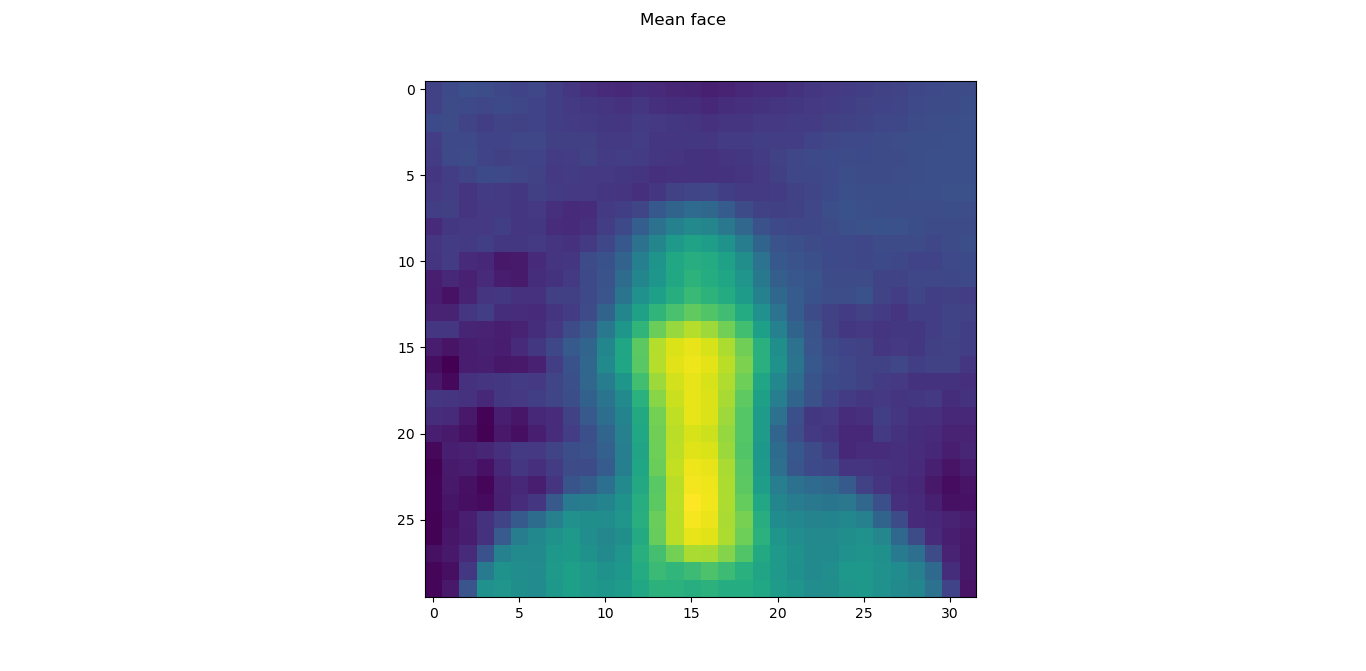
\includegraphics[scale=0.5]{mean_face}
	\caption{Mean face}
	\label{fig:mean_face}
\end{figure}
The first 5 eigen-faces are shown in Fig.\ref{fig:eig_faces}
\newpage
\begin{figure}[h!]
	\centering
	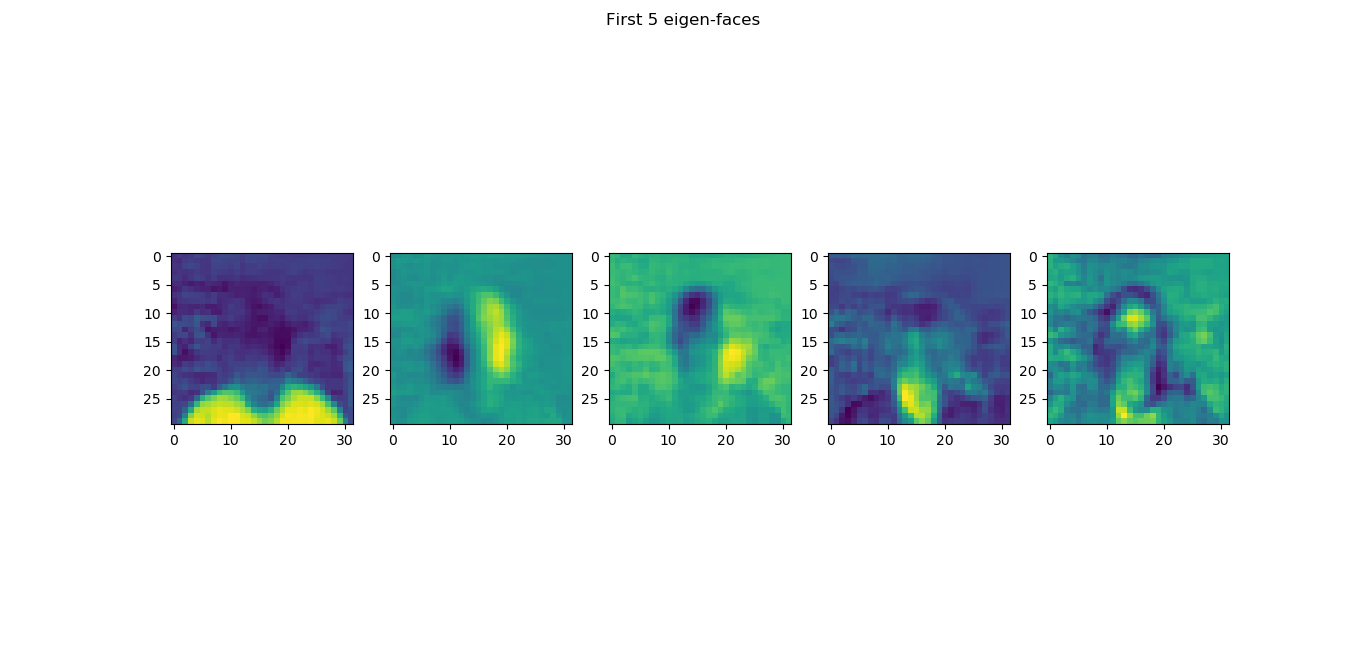
\includegraphics[scale=0.5]{eig_faces}
	\caption{First 5 eigen-faces}
	\label{fig:eig_faces}
\end{figure}
\subsection*{Solution 3.b}
We performed PCA on face training data and found the following proportion of variance plot:
\begin{figure}[h!]
	\centering
	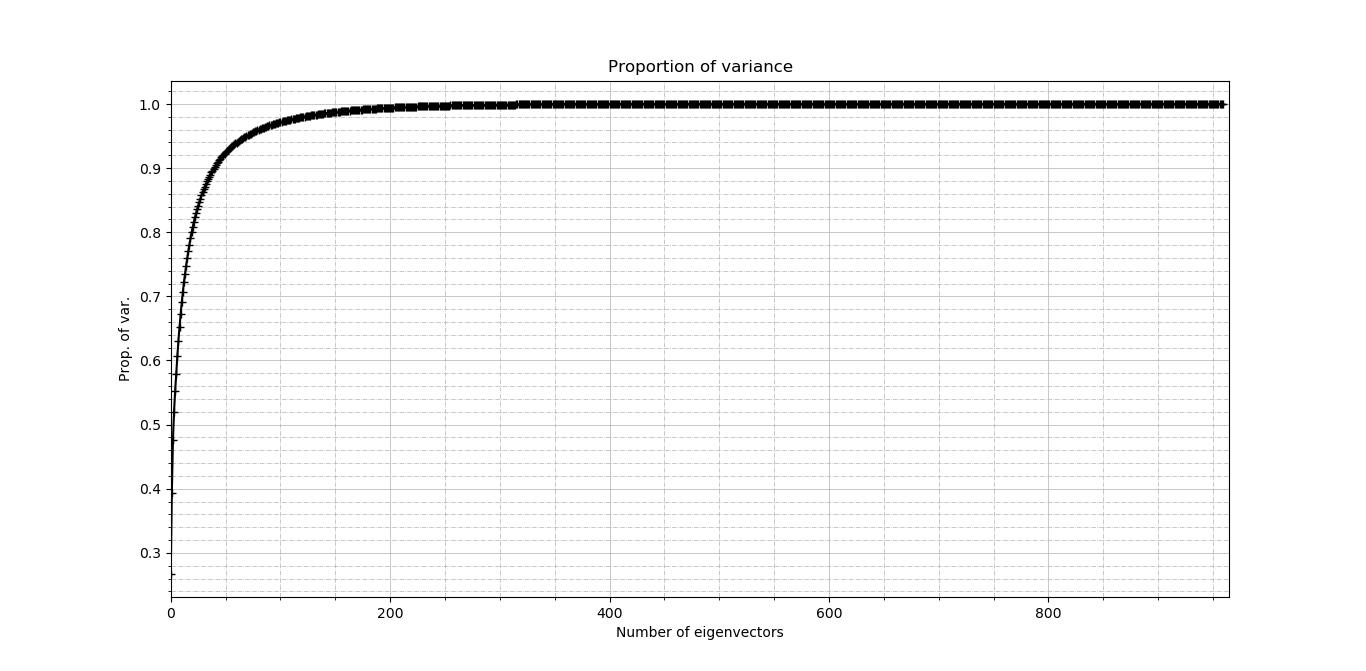
\includegraphics[scale=0.5]{pov_3b}
	\caption{Proportion of variance plot for face training data}
	\label{fig:pov_3b}
\end{figure}
\newline
We can see from Fig.\ref{fig:pov_3b} that the minimum number of eigenvectors that explain at least 90\% of the variance is 40.
\newline
Therefore, we used 40 principal components for PCA and reduced the dimension of the original face data to 40. Then, we used KNN on this reduced dimension face test data. The following table shows the error rates for different k in k-nearest neighbor algorithm on reduced face test data.
\begin{table}[h!]
	\begin{center}
		\begin{tabular}{||c | c | c | c | c ||} 
			\hline
			k & 1 & 3 & 5 & 7 \\ [0.5ex] 
			\hline\hline
			Error rate(\%) & 10.483 & 24.193 & 39.516 & 39.516 \\ [1ex]
			\hline
		\end{tabular}
	\end{center}
	\caption{Q3.b: Error-rate Vs. k table}
\end{table}
\subsection*{Solution 3.c}
\begin{figure}[h!]
	\centering
	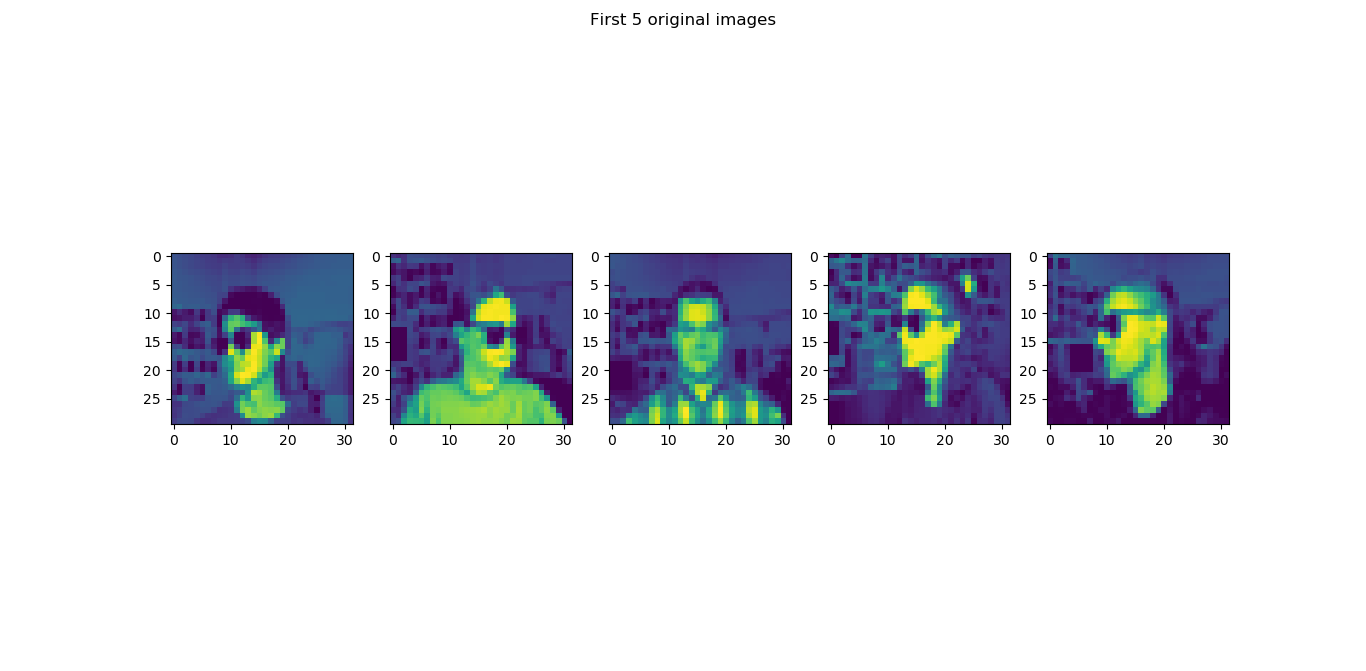
\includegraphics[scale=0.5]{face_orig}
	\caption{Original first 5 faces from training data}
	\label{fig:face_orig}
\end{figure}
\begin{figure}[h!]
	\centering
	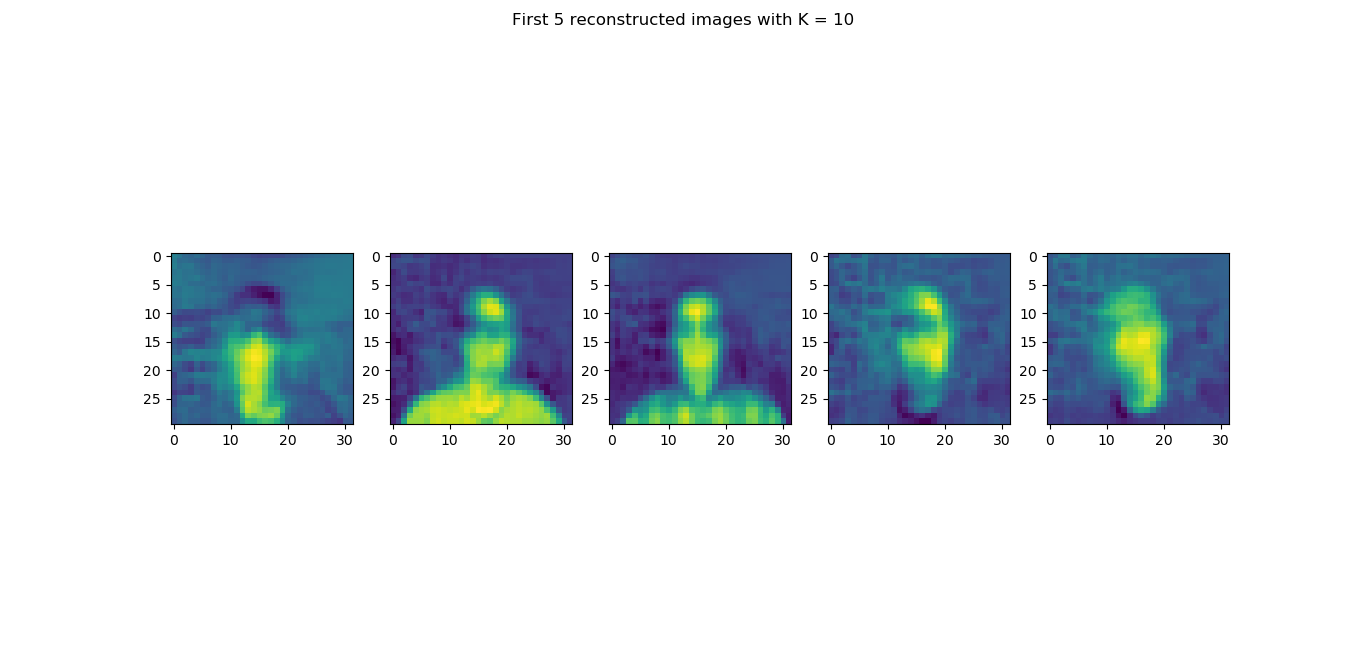
\includegraphics[scale=0.5]{face_pca_10}
	\caption{First 5 reconstructed faces using 10 principal components}
	\label{fig:face_pca_10}
\end{figure}
\begin{figure}[h!]
	\centering
	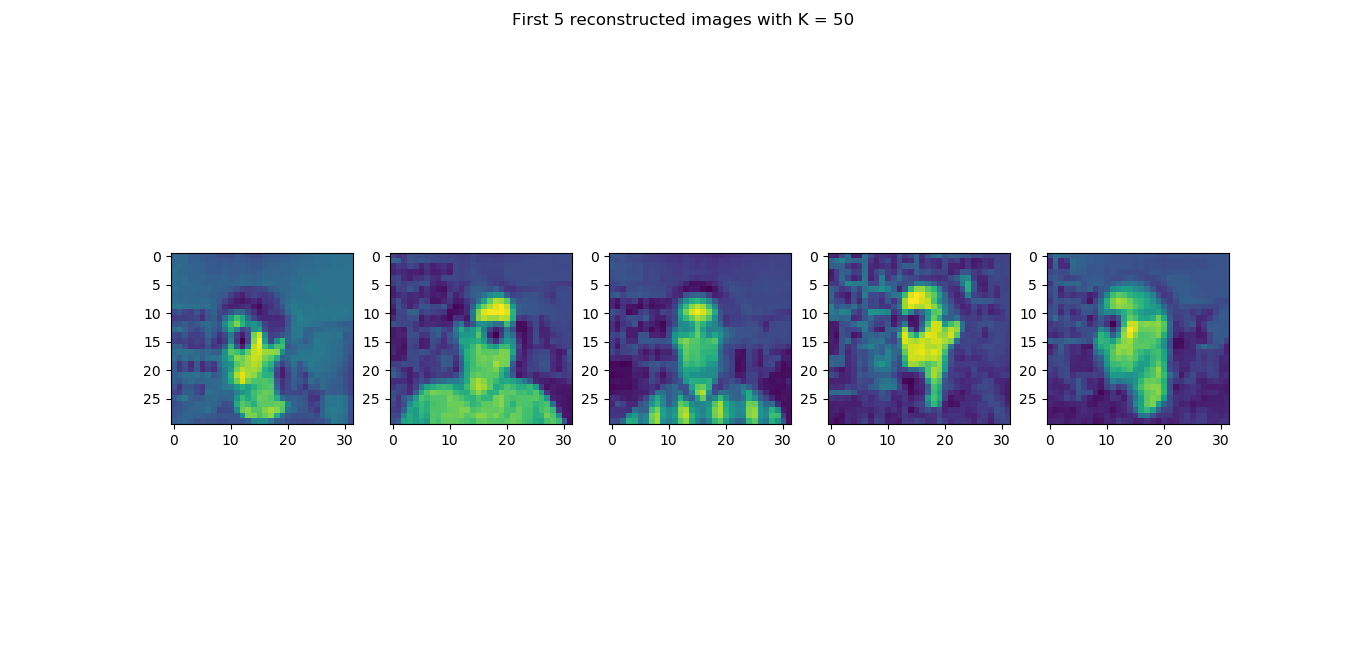
\includegraphics[scale=0.5]{face_pca_50}
	\caption{First 5 reconstructed faces using 50 principal components}
	\label{fig:face_pca_50}
\end{figure}
\begin{figure}[h!]
	\centering
	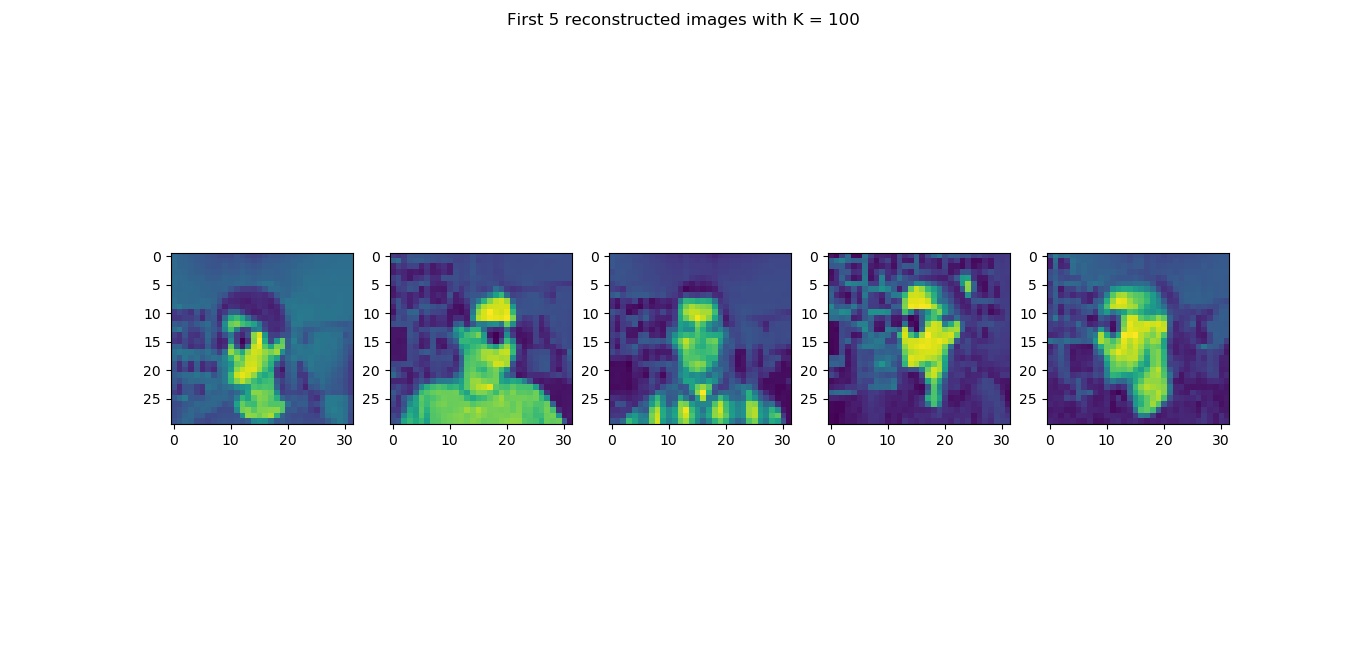
\includegraphics[scale=0.5]{face_pca_100}
	\caption{First 5 reconstructed faces using 100 principal components}
	\label{fig:face_pca_100}
\end{figure}
\newpage
Thus we can see that as we increase the number of principal components, reconstructed images become closer to the original images but at a cost of increased complexity and processing time.
    %\input{problem_2}
    %\input{solution_2}
\end{document}